Во \textbf{введении} определены актуальность темы исследования, степень ее разработанности, цели и задачи диссертационной работы, ее научная новизна, теоретическая и практическая значимость, методология диссертационного исследования, положения, выносимые на защиту, степень достоверности полученных результатов, апробация результатов и личный вклад автора. 

В {\bf главе 1} описан численный метод моделирования течения в трубах. 
%В работе движение жидкости моделируется численными решениями полных трехмерных уравнений Навье-Стокса. 
В предисловии приведен краткий историко-литературный обзор развития численных методов для решения задач гидродинамики и краткий обзор подходов к прямому численному моделированию пристенных турбулентных течений. 

В \textbf{разделе 1.1} приведена постановка задачи. Рассматривается течение вязкой несжимаемой жидкости в прямой трубе круглого сечения. Течение описывается уравнениями Навье-Стокса и неразрывности. На стенке трубы ставится условие прилипания, в продольном направлении --- условие периодичности. Жидкость приводится в движение внешним градиентом давления, определяемым из условия постоянства расходной скорости $U_m$. Постановка задачи традиционна для прямого расчета развитых турбулентных течений в трубах. Задача решается в безразмерных переменных. В качестве основных единиц измерения выступают радиус трубы $R$, удвоенная расходная скорости $U = 2U_m$, равная максимальной скорости в течении Пуазейля, и плотность жидкость $\rho$. Число Рейнольдса $\Re = RU/\nu$, где $\nu$ --- кинематический коэффициент вязкости.

В \textbf{разделе 1.2} описан конечно-разностный метод решения поставленной задачи. Уравнения решаются в цилиндрической системе координат $(x,r,\theta)$. Дискретизация уравнений выполнена на перемежающихся сетках. %, что позволяет удобно аппроксимировать уравнения и граничные условия с сохранением ряда аналогов консервативных свойств исходной системы. 
Ребра сеток совпадают с координатными линиями. Дискретизация по пространственным переменным выполнена со вторым порядком точности. Для интегрирования по времени применен полунеявный метод Рунге-Кутты третьего порядка точности. Наиболее полно метод описан в (Nikitin N. 2006).

\textbf{Раздел 1.3} посвящен практическим вопросам реализации вычислений. Реализованы последовательный и параллельный варианты программы. Расчеты выполнены с использованием оборудования Центра коллективного пользования сверхвысокопроизводительными вычислительными ресурсами МГУ имени М.В.\,Ломоносова. 

В \textbf{разделе 1.4} приведены результаты расчетов движения жидкости в круглой трубе при переходных значениях $\Re$ в достаточно протяженной расчетной области. Турбулентность в расчетах принимает форму локализованных структур, характеристики которых совпадают с характеристиками турбулентных порывов, приведенными в литературе. Это подтверждает адекватность численного метода целям работы и качество его программной реализации. 

На Рисунке \ref{puff_3D_img} изображен турбулентный порыв, рассчитанный при $\Re = 2000$. Светлым и темным тоном представлены области повышенной и пониженной на $0.1U$ скорости относительно течения Пуазейля. Поток направлен слева направо. Протяженность порыва около 30 диаметров трубы, скорость перемещения близка к средней скорости течения. Передняя граница порыва значительно более размыта, чем задняя. Характерной особенностью порыва является наличие центрального ядра с пониженной скоростью и системы вытянутых вдоль потока полос повышенной и пониженной скорости в пристенной области. Сплошность полосчатых структур нарушают значительные по амплитуде случайные по пространственному расположению флуктуации.

\begin{figure}
\center{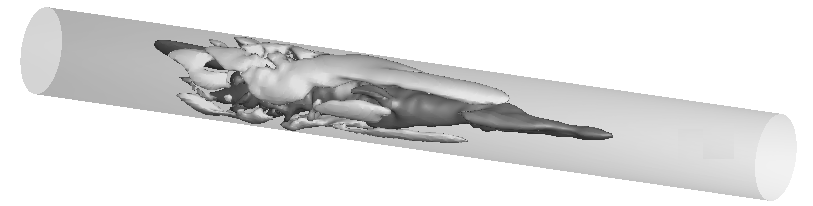
\includegraphics[width=0.9\linewidth]{puff_3D.png}}
\caption{Визуализация численного расчета турбулентного порыва}
\label{puff_3D_img}
\end{figure}
